\chapter{绪论}

\section{研究背景}

量子力学的建立和发展是20世纪人类科学领域最伟大的科学突破之一,它不仅解决了经典物理学在描述微观世界中的失败,而且在许多方面都超越了经典物理学。量子力学的建立不仅推动了物理学的发展,而且对其他学科的发展也产生了深远的影响,许多新兴的领域和学科就此产生,如量子信息科学。

量子信息科学是量子力学和信息科学的交叉领域,它主要研究如何利用量子力学的特性来处理和传输信息。在当今信息时代,信息的处理和传输已经成为人们生活中不可或缺的一部分。
自1940年代,第一台电子计算机诞生以来,计算机技术已经取得了长足的进步,计算机的性能也在不断提高。
英特尔公司创始人戈登·摩尔在1965年提出的摩尔定律,预言单个集成电路上可容纳的晶体管数目每隔18个到24个月就会翻一番。
这一定律不是一个自然定律,而是人们在经验上总结出来的一个规律,但是在过去的几十年中,摩尔定律一直被证明是正确的。但是随着计算机技术的不断发展,集成电路的尺寸越来越小,逐渐接近原子尺度。
在原子尺度下,经典物理学的规律不再适用,量子效应开始显现,这就导致了集成电路的性能难以继续提高,摩尔定律也逐渐失效。

而随着人工智能、大数据、物联网等新兴技术的发展,对计算机性能的需求也越来越高。在这种情况下,传统的计算机技术已经无法满足人们的需求,因此人们开始寻找新的计算机技术。量子计算机作为一种新型的计算机技术,具有很大的发展潜力,并被认为是未来计算机技术的发展方向之一。

在1980年代,Benioff、Manin、Feynman等人提出了量子计算机的概念~\cite{Benioff1980,Benioff1982a,Benioff1982b,Manin1980,Feynman1982}。
最初的动机是希望利用量子力学的特性来模拟量子系统,如果使用经典计算机来模拟量子系统,需要耗费大量的计算资源,而量子计算机可以更加高效地模拟量子系统。后来的研究表明,量子计算机不仅可以模拟量子系统,而且可以解决一些经典计算机难以处理的问题。
1994年,Shor提出了一种基于量子计算机的大整数分解算法~\cite{shor1994algorithms},该算法可以在多项式时间内分解大整数,这对于现代密码学体系具有重要意义。
时至今日,量子计算的研究吸引了众多科学家的关注,也在各个领域衍生出了广泛的应用,包括密码学、量子化学~\cite{peruzzo2014variational, Kandala2017hardware,li2022toward}、量子机器学习~\cite{beer2020training,huang2021experimental,havlivcek2019supervised,mitarai2018quantum}、量子优化算法~\cite{farhi2014quantum,moll2018quantum}等。
此外,除了量子计算之外,量子信息还包括量子纠错、量子复杂度、量子通信、量子传感、量子控制等领域,这些领域也为量子信息科学的发展提供了新的思路和方法。

随着实验技术的进步,量子计算机的实际实现也取得了长足的进步。现在基于各种不同的物理系统,包括离子阱、超导量子比特、量子点、拓扑量子比特等,各种量子计算机的实验平台已经相继建立~\cite{blatt2008quantum,devoret2013superconducting,wallraff2004strong,loss1998quantum}。自2019年以来,研究人员相继在超导量子比特、光量子等平台展示了量子计算在特定任务上对经典计算机的超越,实现了包括随机线路采样~\cite{arute2019quantum}、高斯波色采样等~\cite{zhong2020quantum}等特定任务的量子优越性验证。
近些年来,量子计算机已经发展到了含噪声中等规模量子(Noisy Intermediate-Scale Quantum, NISQ)阶段,这一阶段的量子计算机拥有数十到数百个量子比特,暂无法实现完全容错的量子计算,但是拥有在特定任务上超越经典计算机的潜力。

另一方面,量子计算机的发展也面临着许多困难和挑战。量子计算机的硬件系统非常脆弱,容易受到外界干扰,导致量子比特发生错误。保护量子比特免受外界干扰是量子计算机研究的一个重要课题,量子纠错技术(Quantum Error Correction,QEC)就是为了解决这个问题,通过将量子信息编码在纠错码中,可以有效地保护量子比特免受外界干扰。量子纠错技术是量子计算机研究的一个重要方向,也是实现大规模量子计算的关键技术之一。
噪声阈值定理保证了只要量子比特的错误率低于某个阈值,就可以通过扩大纠错码的规模来实现任意精度的量子计算~\cite{aharonov1996quantum,aliferis2009fault}。
近期,研究人员先后在光量子、超导量子平台上取得了里程碑式的量子纠错实验进展,展示了低于噪声阈值的量子纠错~\cite{reed2012realization,ofek2016extending,riste2015detecting}。
尽管量子计算已经取得了长足的进步,但是要实现大规模量子计算仍然面临着许多困难和挑战,若要真正在生产环境中应用量子计算,还需要解决许多问题,还需要持续在理论和实验方面继续探索和研究。


\section{量子力学简介}
量子力学的建立源于19世纪末20世纪初,当时的物理学家们在研究原子和分子的结构时,发现了一些经典物理学无法解释的现象,如黑体辐射、光电效应、电子的双缝干涉等。20世纪初,普朗克、爱因斯坦、德布罗意、玻尔等人相继提出了量子假设、光量子假设、波粒二象性等概念,奠定了量子力学的基础。
在本节中,我们将简要介绍与量子计算相关的量子力学基础知识,包括量子比特、量子态、量子门、量子纠错等。

\subsection{量子态与密度矩阵}

对于一个纯态量子系统,它在某一时刻的状态可以用一个希尔伯特空间中的一个矢量来表示,称为量子态矢量,利用Dirac符号表示为$|\psi\rangle$。Dirac符号$|\psi\rangle$的数学形式等价于一个N维复线形空间中的列向量,其中N是希尔伯特空间的维度,$|\psi\rangle$称为右矢,代表列向量;$\langle\psi|$称为左矢,代表行向量。两者之间互为共轭转置关系,即$\langle\psi| = |\psi\rangle^\dagger$,其中$\dagger$表示共轭转置。两个量子态之间的内积和外积分别表示为$\langle\psi|\phi\rangle$和$|\psi\rangle\langle\phi|$。

对于一个由$n$个量子比特组成的量子系统,它的状态可以表示为一个$N=2^n$维复数向量,即
\begin{equation}
    |\psi\rangle = \begin{pmatrix} \alpha_0 \\ \alpha_1 \\ \cdots \\ \alpha_{2^n-1} \end{pmatrix} = \sum_{i=0}^{2^n-1} \alpha_i|\phi_i\rangle,
\end{equation}
其中$\alpha_i$是复数,满足$\sum_{i=0}^{2^n-1} |\alpha_i|^2 = 1$,$|\phi_i\rangle$是希尔伯特空间的一组完备的正交归一基矢。
完备性条件$\sum_{i=0}^{2^n-1} |\phi_i\rangle\langle\phi_i| = I$,其中$I$是单位算符。正交性条件$\langle\phi_i|\phi_j\rangle = \delta_{ij}$,其中$\delta_{ij}$是Kronecker delta符号。


对于多个系统构成的复合系统,它的状态可以表示为各个子系统状态的张量积,即
\begin{equation}
    |\psi\rangle = |\psi_1\rangle \otimes |\psi_2\rangle \otimes \cdots \otimes |\psi_n\rangle,
\end{equation}
其中$|\psi_i\rangle$是第$i$个子系统的状态。
因此组合系统中量子态的维度是各个子系统维度的乘积,即$N = N_1 \times N_2 \times \cdots \times N_n$。

对于一个量子系统,它的状态可以是纯态或混合态。纯态是指量子系统处于一个确定的态,可以用上述的矢量来描述;混合态是指量子系统处于一个不确定的态,需要用密度矩阵来描述。密度矩阵是一个厄米矩阵,它可以描述量子系统的统计性质,对于一个纯态量子系统,它的密度矩阵定义为
\begin{equation}
    \rho = |\psi\rangle\langle\psi|,
\end{equation}
其中$|\psi\rangle$是量子系统的状态矢量。对于一个混合态,假设量子系统处于一组纯态$|\psi_i\rangle$的概率为$p_i$,则它的密度矩阵定义为
\begin{equation}
    \rho = \sum_i p_i |\psi_i\rangle\langle\psi_i|,
\end{equation}
其中$p_i$是量子系统处于第$i$个纯态的概率,满足$\sum_i p_i = 1$。
在公理化的量子力学中,密度矩阵满足以下性质:
\begin{enumerate}
    \item 密度矩阵是一个厄米矩阵,即$\rho = \rho^\dagger$;
    \item 密度矩阵是正定的,即对于任意的态矢量$|\psi\rangle$,有$\langle\psi|\rho|\psi\rangle \geq 0$;
    \item 密度矩阵的迹为1,即$\Tr(\rho) = 1$。
\end{enumerate}

对于所有态的均匀混合态,即$\rho = \int d\mu(\lambda) |\lambda\rangle\langle\lambda|$,其中$d\mu(\lambda)$是一个概率测度,满足$\int d\mu(\lambda) = 1$。当概率测度$d\mu(\lambda)$取常用的Haar测度时,这样的密度矩阵称为最大混合态。最大混合态是一个对角矩阵,对角元素都是相等的,即$\rho = \frac{1}{N}I$,其中$N$是希尔伯特空间的维度,$I$是单位算符。
最大混合态常用于描述量子系统的混沌性质,它是量子系统的最大不确定态,对于任意的测量,最大混合态的测量结果是完全随机的。

\subsection{量子态演化}
量子态的演化是量子计算中的一个重要问题,它描述了量子系统在不同时间点的状态之间的关系。在量子力学中,一个封闭系统的演化是由系统的哈密顿量(Hamiltonian)决定的,t时刻的哈密顿量记为$H(t)$,它描述了系统的动力学性质,满足厄米性质$H(t) = H(t)^\dagger$。孤立系统的随时间的演化可以用薛定谔方程(Schrödinger Equation)来描述,即
\begin{equation}
    i\hbar\frac{\partial}{\partial t}|\psi(t)\rangle = H(t)|\psi(t)\rangle,
\end{equation}
其中$\hbar$是约化普朗克常数,$|\psi(t)\rangle$是系统在时间$t$的状态。薛定谔方程的解可以表示为
\begin{equation}
    |\psi(t)\rangle = U(t)|\psi(0)\rangle,
\end{equation}
其中$U(t) = \exp\left(-\frac{i}{\hbar}\int_0^t H(t')dt'\right)$是时间演化算符,它描述了系统从初始状态$|\psi(0)\rangle$到时间$t$的状态$|\psi(t)\rangle$之间的关系。
时间演化算符$U(t)$是一个幺正算符,满足$U(t)U^\dagger(t) = U^\dagger(t)U(t) = I$。


如果采用密度矩阵来描述量子系统,那么密度矩阵的演化可以用薛定谔方程的密度矩阵形式来描述,即
\begin{equation}
    i\hbar\frac{\partial}{\partial t}\rho(t) = [H(t), \rho(t)],
\end{equation}
其中$[\cdot, \cdot]$表示两个算符的对易子。密度矩阵的演化可以表示为
\begin{equation}
    \rho(t) = U(t)\rho(0)U^\dagger(t).
\end{equation}

\subsection{量子测量}
量子测量是量子力学中的一个重要概念,它描述了量子系统在测量过程中的状态演化。在量子力学中,测量是一个不可逆的过程,它会导致量子系统的状态坍缩。在量子力学中,一个量子系统的可观测量是一个厄米算符$O$,满足$O=\sum_i \lambda_i M_i$,其中$\{M_i\}$是一组半正定厄米算符,满足$M_i \geq 0,M_i=M_i^\dagger$和完备性$\sum_i M_i = I$。因为$M_i \geq 0$,所以存在$\{E_i\}$使得$M_i = E_i^\dagger E_i$,这样的测量算符称为正算子(Positive Operator)。
在量子系统的正算子值测量(Positive Operator-Valued Measure, POVM)过程中,量子系统的状态会坍缩到测量结果对应的态上,即
\begin{equation}
    \rho \rightarrow \frac{E_i\rho E_i^\dagger}{\Tr(E_i\rho E_i^\dagger)},
\end{equation}
得到该状态的概率为$p_i = \Tr(E_i\rho E_i^\dagger)$。在测量过程中,测量结果是随机的,但是测量结果的概率是可以计算的。



通常我们关心的是可观测量的测量期望值,它可以表示为$\langle O \rangle$。期望值可以通过对量子态的多次重复测量得到,制备大量相同的量子态,对每个量子态进行测量,然后对测量结果求平均值。对纯态$\ket{\psi}$的可观测量$O$的期望值可以表示为
\begin{equation}
    \langle O \rangle = \langle \psi|O|\psi\rangle=\sum_i \lambda_i p_i=\sum_i \lambda_i \bra{\psi} E_i^\dagger E_i \ket{\psi},
\end{equation}
其中$p_i = \bra{\psi} E_i^\dagger E_i \ket{\psi}$是测量结果为$\lambda_i$的概率。对于混合态$\rho$,可观测量$O$的期望值可以表示为
\begin{equation}
    \langle O \rangle = \Tr(O\rho)=\sum_i \lambda_i \Tr(E_i\rho E_i^\dagger)=\sum_i \lambda_i \Tr(E_i\rho E_i^\dagger).
\end{equation}


\subsection{量子信道}
量子信道是量子信息科学中的一个重要概念,它描述了量子态在开放系统中的演化过程。
对于一个量子系统$A$,如果它与另一个量子系统$B$之间存在相互作用,那么系统$A$的状态会发生演化,这个相互作用可以用一个量子信道来描述。

假设联合系统$AB$的初始状态是$\rho_{AB} = \rho_A \otimes |\psi_0\rangle \langle \psi_0|$,系统$A$的初始状态是$\rho_A = \Tr_B(\rho_{AB})$,系统$B$的初始状态是$\rho_B = \Tr_A(\rho_{AB})=|\psi_0\rangle \langle \psi_0|$。
其中$\Tr_B$表示对系统$B$求偏迹,即对系统$B$的态矢量进行求和,得到系统$A$的密度矩阵;类似的$\Tr_A$表示对系统$A$求偏迹:
\begin{equation}
    \rho_A = \Tr_B(\rho_{AB}) = \sum_i \prescript{}{B}{\langle} \psi_i|\rho_{AB}|\psi_i\rangle_B, \quad \rho_B = \Tr_A(\rho_{AB}) = \sum_j \prescript{}{A}{\langle} \phi_j|\rho_{AB}|\phi_j\rangle_A,
\end{equation}
其中$\{|\psi_i\rangle_B\}$和$\{|\phi_j\rangle_A\}$分别是系统$B$和系统$A$的正交归一基矢。

假设系统$A$和系统$B$之间的相互作用可以用一个幺正算符$U$来描述,系统$A$的状态在相互作用后的状态可以表示为
\begin{equation}
    \rho_A' = \Tr_B(U\rho_{AB}U^\dagger) = \sum_i \prescript{}{B}{\langle} \psi_i|U\rho_{AB}U^\dagger|\psi_i\rangle_B.
\end{equation}

定义 Kraus 算符 $K_i = \prescript{}{B}{\langle} \psi_i|U|\psi_0\rangle_B$,则系统 $A$ 的最终状态可以表示为:
\begin{equation}
    \rho_A' = \sum_i K_i \rho_A K_i^\dagger.
\end{equation}
以上定义的 $K_i$ 满足 $\sum_i K_i^\dagger K_i = \sum_i \prescript{}{B}{\langle} \psi_i|U^\dagger U|\psi_0\rangle_B = I$.

对于一般的量子信道$\mathcal{T}$,可以用一组 Kraus 算符来描述,即
\begin{equation}
    \mathcal{T}(\rho) = \sum_i K_i \rho K_i^\dagger,
\end{equation}
其中 $\sum_i K_i^\dagger K_i = I$。量子信道的作用是将输入态 $\rho$ 映射到输出态 $\mathcal{T}(\rho)$。

Kraus算符保证了量子信道是完全正的,即保证了$\mathcal{T}\otimes I$是正映射,其中$I$是一个恒等算符。假设$\mathcal{T}$有Kraus表示$\mathcal{T}(\rho) = \sum_i K_i \rho K_i^\dagger$,则$\mathcal{T}\otimes I$作用在量子态$\rho=\sum_j \lambda_j \ketbra{\phi_j}$上,有:
\begin{equation}
        \mathcal{T}\otimes I(\rho) = \sum_i (K_i \otimes I)(\rho)(K_i \otimes I)^\dagger = \sum_i (K_i \otimes I)(\sum_j \lambda_j \ketbra{\phi_j})(K_i \otimes I)^\dagger.
\end{equation}
则对于任意的态$\ket{\psi}$,有
\begin{equation}
    \begin{aligned}
        \bra{\psi}(\mathcal{T}\otimes I)(\rho)\ket{\psi} &= \sum_{i,j} \lambda_j \bra{\psi}(K_i \otimes I)\ket{\phi_j}\bra{\phi_j}(K_i \otimes I)^\dagger\ket{\psi} \\
        &= \sum_{i,j} \lambda_j \bra{\psi}(K_i \otimes I)\ket{\phi_j}\bra{\phi_j}(K_i^\dagger \otimes I)\ket{\psi} \\
        &= \sum_{i,j} \lambda_j |\bra{\psi}(K_i \otimes I)\ket{\phi_j}|^2 \geq 0.
    \end{aligned}
\end{equation}
因此,$\mathcal{T}\otimes I$是正的,即$\mathcal{T}$是完全正的。

此外$\sum_i K_i^\dagger K_i = I$保证了量子信道是保迹的,即保证了$\Tr(\mathcal{T}(\rho)) = \Tr(\rho)$。这是因为
\begin{equation}
    \begin{aligned}
        \Tr(\mathcal{T}(\rho)) &= \Tr(\sum_i K_i \rho K_i^\dagger) = \sum_i \Tr(K_i \rho K_i^\dagger) = \sum_i \Tr(\rho K_i^\dagger K_i) \\
        &= \Tr(\rho I) = \Tr(\rho).
    \end{aligned}
\end{equation}

这样完全正的保迹(Completely Positive and Trace-Preserving, CPTP)映射刻画了一般的量子信道的性质,它描述了量子态在开放系统中的演化过程。


\section{量子计算简介}

量子计算是一种基于量子力学原理的计算模型,它利用量子力学的特性来处理和传输信息。
类比经典计算的基本要素如比特、逻辑门、线路等,量子计算也有类似的基本要素。

\subsection{量子比特}
量子比特(Quantum Bit, Qubit)是量子计算的基本单元,它是量子力学中的最小信息单元,类似于经典计算中的比特(Bit)。
经典比特只能处于0或1两种状态,而量子比特可以处于0和1的叠加态,这通常是对应于二能级量子系统、或是多能级量子系统的两个特定的能级。
为了方便将两个能级记为$|0\rangle$和$|1\rangle$。在矩阵表示中,$|0\rangle$和$|1\rangle$分别表示为
\begin{equation}
    |0\rangle = \begin{pmatrix} 1 \\ 0 \end{pmatrix}, \quad |1\rangle = \begin{pmatrix} 0 \\ 1 \end{pmatrix}.
\end{equation}

一个任意量子比特的状态可以表示为
\begin{equation}
    |\psi\rangle = e^{i\gamma}(\cos\frac{\theta}{2}|0\rangle + e^{i\phi}\sin\frac{\theta}{2}|1\rangle)=e^{i\gamma}\begin{pmatrix}
        \cos\frac{\theta}{2} \\ e^{i\phi}\sin\frac{\theta}{2}
    \end{pmatrix},
\end{equation}
其中$\theta$和$\phi$是两个角度,$\gamma$是一个全局相位,满足$0 \leq \theta \leq \pi$,$0 \leq \phi < 2\pi$,$0 \leq \gamma < 2\pi$。 量子比特的状态可以用Bloch球来表示,Bloch球是一个单位球,它的表面上的点对应于量子比特的状态。

一个由n个量子比特组成的量子系统有$2^n$个本征态,它的状态可以用长度为n的二进制串来表示,即$|x_1x_2\cdots x_n\rangle$,其中$x_i \in \{0, 1\}$。一个n量子比特的量子系统的状态可以表示为
\begin{equation}
    |\psi\rangle = \sum_{x=0}^{2^n-1} \alpha_x |x_1x_2\cdots x_n\rangle,
\end{equation}
其中$\alpha_x$是复数,满足$\sum_{x=0}^{2^n-1} |\alpha_x|^2 = 1$。
有时也会使用十进制表示,即$|x\rangle$,其中$x \in \{0, 1, \cdots, 2^n-1\}$。这样的基矢称为计算基矢(Computational Basis)。

\subsection{量子线路}
量子线路是量子计算中的一个重要概念,它描述了量子比特之间的相互作用关系。量子线路由量子门(Quantum Gate)组成,量子门是用来操作量子比特的基本单元,类似于经典计算中的逻辑门。量子门是一个幺正算符,它作用在量子比特上,改变量子比特的状态。

最简单的一类门是单比特量子门,常见的单比特量子门有Pauli门、Hadamard门、相位门、T门等。Pauli门是一组三个单比特门,分别是$X$门、$Y$门和$Z$门,它们的矩阵表示分别为
\begin{equation}
    X = \begin{pmatrix} 0 & 1 \\ 1 & 0 \end{pmatrix}, \quad Y = \begin{pmatrix} 0 & -i \\ i & 0 \end{pmatrix}, \quad Z = \begin{pmatrix} 1 & 0 \\ 0 & -1 \end{pmatrix}.
\end{equation}
Hadamard门是一个单比特门,常用于产生均匀叠加态,它常简记为H门,其矩阵表示为
\begin{equation}
    H = \frac{1}{\sqrt{2}}\begin{pmatrix} 1 & 1 \\ 1 & -1 \end{pmatrix}.
\end{equation}
上述的门矩阵表示既是幺正也是厄米的,因此既可以作为量子门,也可以作为测量算符。
另外还有两个常用的单比特门,分别是相位门(简记为$S$),还有T门,其矩阵表示分别为
\begin{equation}
    S = \begin{pmatrix} 1 & 0 \\ 0 & i \end{pmatrix}, \quad T = \begin{pmatrix} 1 & 0 \\ 0 & e^{i\pi/4} \end{pmatrix}.
\end{equation}

此外还有一类常用的含参数的单比特门,称为单比特旋转门,它们的矩阵表示为
\begin{equation}
    \begin{aligned}
        &R_X(\theta) =e^{-i\frac{\theta}{2}X} = \begin{pmatrix} \cos\frac{\theta}{2} & -i\sin\frac{\theta}{2} \\ -i\sin\frac{\theta}{2} & \cos\frac{\theta}{2} \end{pmatrix}, \\ &R_Y(\theta)=e^{-i\frac{\theta}{2}Y} = \begin{pmatrix} \cos\frac{\theta}{2} & -\sin\frac{\theta}{2} \\ \sin\frac{\theta}{2} & \cos\frac{\theta}{2} \end{pmatrix},\\ &R_Z(\theta)=e^{-i\frac{\theta}{2}Z} = \begin{pmatrix} e^{-i\theta/2} & 0 \\ 0 & e^{i\theta/2} \end{pmatrix}.
    \end{aligned}
\end{equation}
这些门可以通过旋转Bloch球来实现,从几何的角度,他们分别是将量子比特绕Bloch球的X轴、Y轴、Z轴旋转一个角度$\theta$。实际上,任意的单比特门都可以视为在Bloch球上的一个旋转操作,有如下的表示
\begin{equation}
    U = e^{i\alpha}R_n(\theta),
\end{equation}
其中$e^{i\alpha}$是一个全局相位,$R_n(\theta)$是绕Bloch球上的一个单位向量$n$旋转一个角度$\theta$,满足
\begin{equation}
    R_n(\theta) = \cos\frac{\theta}{2}I - i\sin\frac{\theta}{2}n\cdot\vec{\sigma},
\end{equation}
其中$\vec{\sigma} = (\sigma_x, \sigma_y, \sigma_z)$是Pauli矩阵向量,$n$是一个单位向量,满足$n\cdot n = 1$。
通过欧拉角分解,任意的旋转都可以表示为三个旋转门的乘积,即
\begin{equation}
    R_n(\theta) = R_Z(\beta)R_Y(\gamma)R_Z(\delta).
\end{equation}
因此,只使用两种轴的旋转门就可以实现任意的单比特门。

除了单比特门之外,还有多比特门,常见的多比特门有CNOT门。CNOT门是一个两比特门,它的矩阵表示为
\begin{equation}
    \text{CNOT} = \ketbra{0}{0}\otimes I + \ketbra{1}{1}\otimes X=\begin{pmatrix} 1 & 0 & 0 & 0 \\ 0 & 1 & 0 & 0 \\ 0 & 0 & 0 & 1 \\ 0 & 0 & 1 & 0 \end{pmatrix}.
\end{equation}

单比特旋转门的推广是多比特旋转门。为了介绍多比特旋转门,我们首先介绍Pauli word的概念。Pauli word是由Pauli算符$X$、$Y$、$Z$以及单位算符$I$进行张量积组成的一个算符,例如$XIY$、$ZZI$等。形式化地,一个长度为n的Pauli word可以表示为
\begin{equation}
    P = \bigotimes_{i=1}^n P_i,
\end{equation}
其中$P_i \in \{I, X, Y, Z\}$。
一个n-qubit的多比特旋转门是Pauli word的指数函数,即
\begin{equation}
    R_P(\theta) = e^{-i\frac{\theta}{2} P},
\end{equation}
其中$P$是一个长度为n的Pauli word,$\theta$是旋转角度。
多比特旋转门在一大类被称为变分量子算法(Variational Quantum Algorithm,VQA)中扮演着重要的角色。
多比特旋转门的实现略显复杂,但是可以通过一系列的单比特门和CNOT门来实现。

在一个量子系统中,如果能够实现任意的单比特门和CNOT门,那么这个量子系统就是通用量子计算机,可以实现任意的幺正操作。在一些特定的量子计算系统中,旋转门的实现可能会受到限制,并且旋转门的实现可能使得量子纠错变得更加困难。因此,还有一种常见的办法是使用一组固定的门集合,使得这个门集合可以实现任意的幺正操作,这样的门集合称为通用量子门集合。

常见的通用量子门集合有Clifford+T门集合。
Clifford门是一类幺正门,它们保持Pauli算符的对易关系,即对于任意的Pauli算符$P$和Clifford门$C$,有$CPC^\dagger = P'$,其中$P'$也是一个Pauli算符。Clifford门的特点是它们可以通过Hadamard门、相位门、CNOT门来构造。

将量子门按照一定的顺序组合起来,就构成了一个量子线路。量子线路是量子计算中的一个重要概念,它描述了量子比特之间的相互作用关系。量子线路由量子门组成,量子门是用来操作量子比特的基本单元,类似于经典计算中的逻辑门。量子线路的输入是一个初始的量子态,输出是一个最终的量子态。量子线路的运行过程是一个量子态在量子门作用下的演化过程,它描述了量子比特之间的相互作用关系。图~\ref{fig:quantum-circuit}展示了一个量子线路的示意图,其中包含两个被初始化为$|0\rangle$的量子比特,通过Hadamard门和CNOT门的作用,最终的量子态会被测量。

\begin{figure}[h]
    \centering
    \begin{quantikz}
        \lstick{$|0\rangle$} & \gate{H} & \ctrl{1} & \meter{} \\
        \lstick{$|0\rangle$} & \qw & \targ{} & \meter{} \\
    \end{quantikz}
    \caption{量子线路示意图}\label{fig:quantum-circuit}
\end{figure}


\subsection{量子噪声}
在实际的量子计算中,量子比特会受到噪声的影响,这会导致量子计算的结果出现误差。量子噪声是量子计算中的一个重要问题,可以通过量子信道来描述。常见的噪声分为两类,一类是保持最大混合态的噪声,另一类是保持最大纯态的噪声。

\section{张量网络图}


张量网络图记号作为一种直观的数学工具,通过几何拓扑结构将复杂的张量运算转化为可视化的图形操作。其核心思想是将张量的每个自由度(指标)表示为连接节点的“腿”(leg),张量间的缩并操作则通过腿的连接实现。

张量网络图记号的发展与量子多体物理和量子信息科学密切相关。20世纪90年代,White提出的密度矩阵重整化群(DMRG)方法首次隐式地使用了张量网络的拓扑结构。2003年,F. Verstraete等人明确提出矩阵乘积态(MPS)的图表示,标志着张量网络图记号的形式化。


在张量网络图记法中,向量作为一阶张量,可通过单个节点及其左侧延伸的线段表示:
\begin{equation}
  \ket{v}
  =
  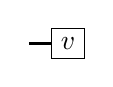
\begin{tikzpicture}[baseline=(current bounding box.center)]
    \node[draw] (s0) at (0,0) {$v$};
    \draw [thick] (-0.5,0)--(s0);
  \end{tikzpicture},
\end{equation}
其中$v=\begin{pmatrix} v_1 \\ v_2 \\ \vdots \\ v_n \end{pmatrix}$。
当给腿赋予指定的指标时,可以获得所表示向量的分量:
\begin{equation}
  \braket{i}{v}
  =v_i=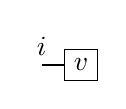
\begin{tikzpicture}
    \node[draw] (s0) at (0,0) {$v$};
    \draw [thick] (-0.5,0)--(s0);
    \node[above] at (-0.5,0) {$i$};
  \end{tikzpicture}
\end{equation}


矩阵在张量网络图中作为二阶张量,可以被表示为具有左右两侧连线的节点:
\begin{equation}
  A
  =
  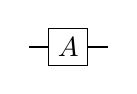
\begin{tikzpicture}[baseline=(current bounding box.center)]
    \node[draw] (s0) at (0,0) {$A$};
    \draw [thick] (-0.5,0)--(s0) (s0)--(0.5,0);
  \end{tikzpicture},
\end{equation}
其中$A=\begin{pmatrix} a_{11} & a_{12} \cdots \\ a_{21} & a_{22} \cdots \\ \vdots & \vdots \end{pmatrix}$。
矩阵的元素可通过指定连接的腿的指标获得:
\begin{equation}
  a_{ij}=
  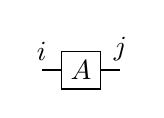
\begin{tikzpicture}[baseline=(current bounding box.center)]
    \node[draw] (s0) at (0,0) {$A$};
    \draw [thick] (-0.5,0)--(s0) (s0)--(0.5,0);
    \node[above] at (-0.5,0) {$i$};
    \node[above] at (0.5,0) {$j$};
  \end{tikzpicture}
\end{equation}


由矩阵的张量网络图表示,矩阵的转置操作可通过旋转张量对应的连接方向实现:
\begin{equation}
  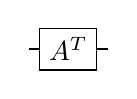
\begin{tikzpicture}[baseline=(current bounding box.center)]
    \node[draw] (s0) at (0,0) {$A^T$};
    \draw [thick] (-0.5,0)--(s0) (s0)--(0.5,0);
  \end{tikzpicture}
  =
  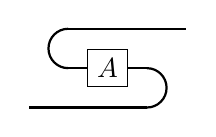
\begin{tikzpicture}[baseline=(current bounding box.center)]
    \node[draw] (s0) at (0,0) {$A$};
    \draw[thick] (-0.5,0)--(s0) (s0)--(0.5,0);
    \draw[thick] (-0.5,0.5) arc(90:270:0.25);
    \draw[thick] (0.5,-0.5) arc(-90:90:0.25);
    \draw[thick] (-0.5,0.5)--(1,0.5) (0.5,-0.5)--(-1,-0.5);
  \end{tikzpicture}
\end{equation}

对于矩阵的乘法操作,在张量网络图中是由连接相邻张量的对应边实现指标收缩来表示:
\begin{equation}
  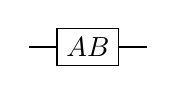
\begin{tikzpicture}[baseline=(current bounding box.center)]
    \node[draw] (s1) at (0,0) {$AB$};
    \draw [thick] (-0.75,0)--(s1) (s1)--(0.75,0);
  \end{tikzpicture}
  =
  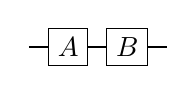
\begin{tikzpicture}[baseline=(current bounding box.center)]
    \node[draw] (s0) at (0,0) {$A$};
    \node[draw] (s1) at (0.75,0) {$B$};
    \draw [thick] (-0.5,0)--(s0) (s0)--(s1) (s1)--(1.25,0);
  \end{tikzpicture}
\end{equation}
这是因为矩阵乘法的元素表达式为
\begin{equation}
  (AB)_{ij}=\sum_k A_{ik}B_{kj}=\sum_k
  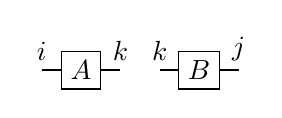
\begin{tikzpicture}[baseline=(current bounding box.center)]
    \node[draw] (s0) at (0,0) {$A$};
    \node[draw] (s1) at (1.5,0) {$B$};
    \draw [thick] (-0.5,0)--(s0) (s0)--(0.5,0) (s1)--(2,0) (s1)--(1,0);
    \node[above] at (-0.5,0) {$i$};
    \node[above] at (0.5,0) {$k$};
    \node[above] at (1,0) {$k$};
    \node[above] at (2,0) {$j$};
    \end{tikzpicture}=
    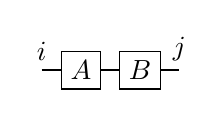
\begin{tikzpicture}[baseline=(current bounding box.center)]
        \node[draw] (s0) at (0,0) {$A$};
        \node[draw] (s1) at (0.75,0) {$B$};
        \draw [thick] (-0.5,0)--(s0) (s0)--(s1) (s1)--(1.25,0);
        \node[above] at (-0.5,0) {$i$};
        \node[above] at (1.25,0) {$j$};
    \end{tikzpicture}
\end{equation}





除了矩阵的乘法,另一种常见的张量积操作,在张量网络图中被表示为为张量的垂直堆叠:
\begin{equation}
  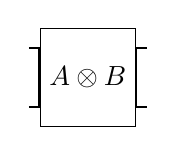
\begin{tikzpicture}[baseline=(current bounding box.center)]
    \node[draw,minimum height=1.25cm] (s1) at (0,0) {$A\otimes B$};
    \draw [thick] (-0.75,0.375)-|(s1.west) (-0.75,-0.375)-|(s1.west) (s1.east)|-(0.75,0.375) (s1.east)|-(0.75,-0.375);
  \end{tikzpicture}
  =
  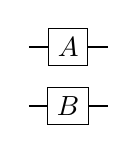
\begin{tikzpicture}[baseline=(current bounding box.center)]
    \node[draw] (s0) at (0,0) {$A$};
    \node[draw] (s1) at (0,-0.75) {$B$};
    \draw [thick] (-0.5,0)--(s0)--(0.5,0)  (-0.5,-0.75)--(s1)--(0.5,-0.75);
  \end{tikzpicture}
\end{equation}


矩阵的迹运算可以通过将张量的对应边连接并收缩来表示:
\begin{equation}
  \Tr{A}
  =
  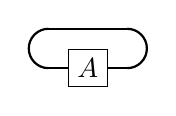
\begin{tikzpicture}[baseline=(current bounding box.center)]
    \node[draw] (s0) at (0,0) {$A$};
    \draw [thick] (-0.5,0)--(s0) (s0)--(0.5,0);
    \draw[thick] (-0.5,0.5) arc(90:270:0.25);
    \draw[thick] (0.5,0) arc(-90:90:0.25);
    \draw [thick] (-0.5,0.5)--(0.5,0.5);
  \end{tikzpicture}
\end{equation}

上述图记号通过几何拓扑直观反映了张量运算的代数结构,特别在处理高维张量收缩时,能有效降低传统指标记法的复杂性。后续章节将基于此记号体系,介绍Pauli路径积分算法的张量网络图表示。


\section{本章小结}
本章介绍了量子信息科学的基本概念,包括量子信息科学的研究背景、量子力学的基本知识、量子计算的基本概念等。介绍了表示量子系统状态的纯态、混合态、密度矩阵的概念,接着介绍了量子态的演化、量子测量的概念。最后介绍了量子计算的基本概念,包括量子比特、量子线路、量子门等。本章的内容为后续章节的内容打下了基础。

在后面的章节中,我们将介绍
%#TODO